\documentclass[fleqn]{jbook}
\usepackage{physpub}

\begin{document}

\begin{question}{専攻 問題9}{}

生体物質は光吸収や蛍光発光を用いて、解析することが多い。電子の質量をm、光速度をc、プランク定数をhとして、以下の問いに答えよ。

\begin{subquestions}
\SubQuestion
図のような動物の目のレチナール様視物質Aの光吸収を論じる。

\begin{center}
\includegraphics[clip,height=25mm,width=78mm]{1997phy9-1.eps}
\end{center}

\begin{subsubquestions}
\SubSubQuestion
電子の励起状態を求めよ。但し視物質のポリエン鎖(長さL)を一次元的に動く炭素原子の$\pi$電子が光を吸収するとして考える。電子はこのLの部分の外には出られない。長さLのポリエン鎖内の各々の炭素原子は1個の$\pi$電子を供給する。

\SubSubQuestion
炭素原子の何軌道が$\pi$電子軌道を形成するのか。

\SubSubQuestion
L=1nmとするとき、光吸収の波長を求めよ。但しmc/h=412nm$^{-1}$を用いよ。

\SubSubQuestion
我々が夕闇の中でも目が見えるようにするには、視物質Aの構造をどう変化させればよいかを論じよ。
\end{subsubquestions}

\SubQuestion
蛍光性アミノ酸の光学的性質は環状化合物ベンゼンをモデルとして理解できる。ベンゼンの光吸収も前問と同様に、C-C結合上を自由に動ける$\pi$電子の吸収として考えて、光吸収の波長を求めよ。但しこの場合、電子は円周がベンゼンの周囲の長さに等しいとした半径rの円周軌道上を動くと考えてよい。C-C結合の長さは0.14nmとせよ。

\SubQuestion
環状炭化水素化合物Fは、図のように基底電子準位S$_0$と第一励起準位S$_1$を持ち、更にこれらS$_0$とS$_1$の上に振動準位を持つ。

\begin{subsubquestions}
\SubSubQuestion
Fが孤立して真空中にあるとき、吸収と蛍光発光の強度スペクトルを書き込め。但し最初は電子はすべてS$_0$準位に居るとする。

\SubSubQuestion
Fを有機溶媒にとかすと、スペクトルはどう変化するか書き込め。

\SubSubQuestion
S$_1$励起準位に近い励起準位を持つ重金属を溶液に混在させると、Fの蛍光はどう変化するか?理由も書け。
\vspace{5mm}
\begin{center}
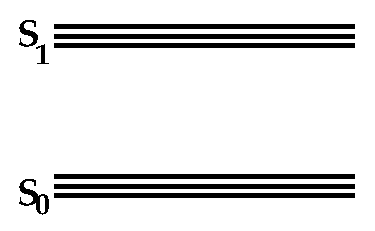
\includegraphics[clip,height=25mm,width=35mm]{1997phy9-2.eps}
\hspace{20mm}
\includegraphics[clip,height=25mm,width=43mm]{1997phy9-3.eps}
\end{center}
\end{subsubquestions}

\parbox[t]{100mm}{
\SubQuestion
蛍光性アミノ酸であるトリプトファンの蛍光を用いて水溶性球状タンパク質Pの存在状態を測定する。Pの水溶液に塩酸グアニジンを加えていったとき、トリプトファンの蛍光が図のように低下した。

\begin{subsubquestions}
\SubSubQuestion
濃度C$_0$の前後でPの構造にどのような変化が起こっているか。

\SubSubQuestion
濃度C$_0$の前後でトリプトファンの蛍光スペクトルはどのように変化するか。
\end{subsubquestions}
}\parbox[t]{60mm}{
\begin{center}
\includegraphics[clip,height=30mm,width=50mm]{1997phy9-4.eps}
\end{center}
}
\end{subquestions}
\end{question}
\begin{answer}{専攻 問題9}{}

\begin{subanswers}
\SubAnswer

\begin{subsubanswers}
\SubSubAnswer
1つの電子に注目すると、$x<0,L<x$で$V=+\infty$、$0\le x\le L$で$V=0$の井戸型
ポテンシャルと考えて$0\le x\le L$のシュレディンガー方程式は
\[
\frac{-\hbar^2}{2m}\Deriver{^2}{x^2}\Psi(x)=E\Psi(x)
\]
$2mE/\hbar^2=k^2$とおくと、$\Psi(0)=0$より$\Psi(x)=A\sin kx$。
$\Psi(L)=0$より$kL=n\pi \quad (n=1,2,...)$。よって、
\parbox[t]{100mm}{
\[
E=\frac{\hbar^2}{2m}\left(\frac{\pi n}{L}\right)^2=\frac{h^2n^2}{8mL^2}\qquad (n=1,2,...)
\]
\[
\Psi(x)=A\sin \frac{n\pi}{L}x
\]
係数Aは規格化条件より決める。
\[
A^2\int_0^L\sin^2 \frac{n\pi x}{L}dx=A^2\int_0^L\frac{1-\cos \frac{2n\pi x}{L}}
{2}dx=A^2\frac{L}{2}=1
\]
\[
A=\sqrt{\frac{2}{L}}
\]
ポリエン鎖の中に10個の電子が詰まっている。$n=1$準位から順に電子を詰めていくと
$n=6$が励起状態になる。}\parbox[t]{60mm}
{
\begin{center}
\includegraphics[clip,height=40mm,width=50mm]{1997phy9-5.eps}
\end{center}
}

よって励起状態の波動関数は
\[
\Psi(x)=\sqrt{\frac{2}{L}}\sin \frac{6\pi }{L}x
\]
%
\SubSubAnswer
p軌道
%
\SubSubAnswer
$E=h\nu=h\frac{\lambda}{c}$より$n=5$から$n=6$への遷移のときに吸収される
エネルギーは
\[
\frac{h^2}{8mL^2}(6^2-5^2)=h\frac{c}{\lambda}
\Longrightarrow
\lambda=\frac{8mc}{h}L^2\frac{1}{11}=\frac{8\times 412[{\Unit{nm}}^{-1}]
\times (1[{\Unit{nm}}^2])}{11}=3.00\times 10^2[{\Unit{nm}}]
\]


\SubSubAnswer
C=Cの長さを$a$(但し、C-Cも同じ程度として計算する。)、共役電子系の電子の電子数を$n$とすると、$L \sim (n-1)a$であり、HOMOは$n/2$の準位で、LUMOは$n/2+1$の準位であるから、
\[
\lambda \sim \frac{8mc}{h}\frac{\{(n-1)a\}^2}{\{(\frac{n}{2})+1\}^2-(\frac{n}{2})^2} = \frac{8mc}{h}a^2 \frac{(n-1)^2}{n+1} \sim 40.1 \times \frac{(n-1)^2}{n+1} [\Unit{nm}]
\]
 
$n$が十分大きいならば、$\lambda \propto n \propto L$なので、Aの鎖の部分が伸びればより長い波長の光を見られるようになるから、赤外線が見える程度まで伸びればよい。

{\bf{ [補足]}}
視物質は、色素タンパク質として、レチナールを含んでいる。レチナールは、それを取り囲むタンパク質オプシンのアミノ酸残基の一つであるリジン残基のアミノ酸と、シッフ残基で結合している。レチナールの吸収極大波長は、近紫外部の$370{\Unit{[nm]}}$付近であるが、それがシッフ塩基結合を作り、その結合にプロトンが配位すると、吸収極大部は$400\Unit{[nm]}$に移る。視物質の色は、$340\Unit{[nm]}$から、$640\Unit{[nm]}$付近にまでわたっている。これらの吸収極大波長は、一部に発色団の修飾によって、大部分はタンパク質オプシンの発色団近傍のアミノ酸残基の違いによって決まっていると考えられる。
\end{subsubanswers}

%%
\SubAnswer
円周の長さは$L=6\times 0.14=0.84[\Unit{nm}]$\\
この場合、シュレディンガー方程式は問題1と同じで境界条件を$\Psi(0)=\Psi(L)$
とする。すると$kL=2\pi n \quad (n=0,\pm 1,\pm 2,...)$
\[
E=\frac{h^2n^2}{2mL^2}\qquad (n=0,\pm 1, \pm 2,...)
\]
\parbox[t]{60mm}{
\begin{center}
\includegraphics[clip,height=40mm,width=50mm]{1997phy9-6.eps}
\end{center}
}\parbox[t]{100mm}{$\pi$電子は6個あるので、$n=0$のみが、一重縮退で、ほかの軌道は、2重縮退していることに注意して、$n=0$から順に電子を詰めていくと、$n=\pm 2$が励起状態である。
\[
\frac{h^2}{2mL^2}\{(\pm 2)^2-(\pm 1)^2\}=h\frac{c}{\lambda}
\]
\[ \hspace{-13mm}\Yueni
\lambda=\frac{2mc}{h}L^2\frac{1}{3}=\frac{2\times 412[{\Unit{nm}}^{-1}]
\times 0.84[{\Unit{nm}}^2]}{3}=1.9\times 10^2 [{\Unit{nm}}]
\]
}

%%
\SubAnswer
\begin{subsubanswers}
\SubSubAnswer

\parbox[t]{60mm}{まずfig.3,fig.4より、無輻射遷移により振動の基底状態に
遷移してから蛍光を発することに注意する({\bf{[補足1]}}参照)と、スペク
トルの数は、吸収、蛍光ともに3本であり、波長は図の符合を用いて、ウ$<$
イ$<$ア$=$カ$<$オ$<$エとなる。}
\parbox[t]{50mm}{
\begin{center}
\includegraphics[clip,height=35mm,width=40mm]{1997phy9-7.eps}
\end{center}}
\parbox[t]{50mm}{\vspace*{-5mm}
\begin{center}
\includegraphics[clip,height=40mm,width=40mm]{1997phy9-8.eps}
\end{center}}

\parbox[t]{60mm}{\vspace*{-10mm}
\begin{center}
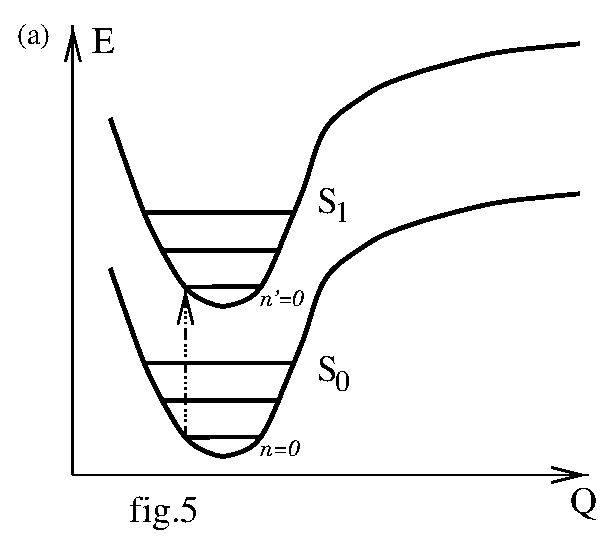
\includegraphics[clip,height=45mm,width=50mm]{1997phy9-9.eps}
\end{center}}\parbox[t]{100mm}{fig.5($Q$は基準振動座標)のように励起状態のポテンシャル曲線が基底状態と似ており、平衡基準振動座標もほぼ同じである場合は、基底状態の振動準位を$n$、励起状態の振動準位を$n'$とすれば、$(n,n')=(0,0)$の波動関数の重なり積分が大きく、0-0遷移が可能となるが、$n'=1,2$となるにつれて、波動関数の重なりが悪くなるため、強度が落ちる。}

\parbox[t]{60mm}
{fig.6のように励起状態の平衡基準振動座標が基底状態とずれている場合、波動関数の重なりは、$(n,n')=(0,1)$が一番大きくなる。同様に、fig.7のようなポテンシャル曲線のシフトも考えることもでき、強度についても、同じような考察ができる。
}\hspace{-7mm}\parbox[t]{120mm}
{\vspace*{-10mm}
\begin{center}
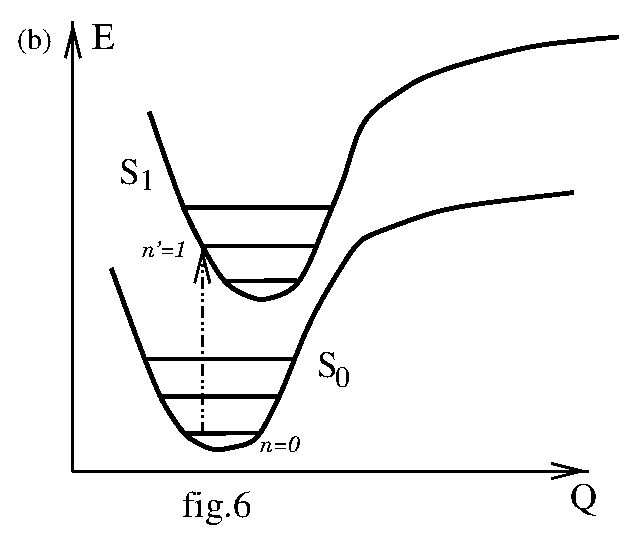
\includegraphics[clip,height=45mm,width=50mm]{1997phy9-10.eps}
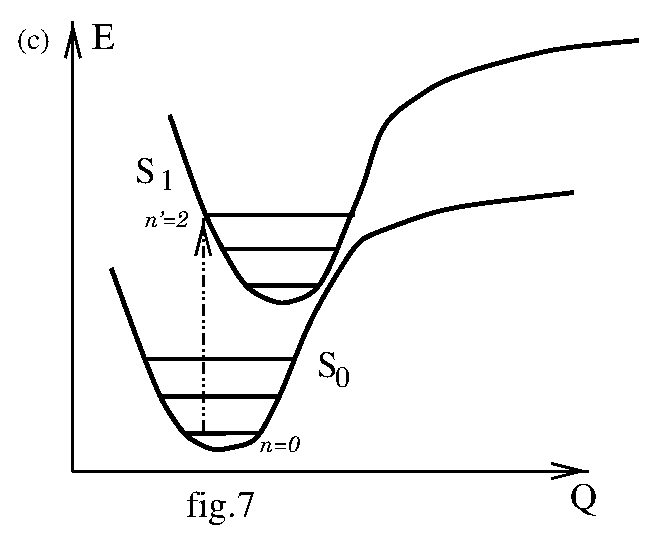
\includegraphics[clip,height=45mm,width=50mm]{1997phy9-11.eps}
\end{center}}

以上を、まとめると、下のようになる。振動数-強度の関係のグラフを書けば、
吸収スペクトルが、蛍光スペクトルの鏡像関係にあることに、注意されたい。
\begin{center}
\includegraphics[clip,height=35mm,width=40mm]{1997phy9-12.eps}
\hspace{5mm}
\includegraphics[clip,height=35mm,width=40mm]{1997phy9-13.eps}
\hspace{5mm}
\includegraphics[clip,height=35mm,width=40mm]{1997phy9-14.eps}
\end{center}

{\bf{[補足1]}}蛍光過程の時間(アンサンブル平均としての寿命)は、今の場
合、近紫外を考え、約10$^{-9}$[{\Unit{s}}]である。第一励起状態の第一振
動準位や第二振動励起準位から、発光しないわけではないが、振動緩和(無輻
射遷移)の時間が約10$^{-12}$[{\Unit{s}}]であるため、振動緩和と発光が競
争し、1000個に1つの割合でしか発光しないことになる。そのため、事実上、
第0振動準位のみ考えれば良い。

一方、『電子遷移の前後で分子は形を変えない』というFranck-Condonの原理
があるが、この原理は、1つの電子に注目し、その電子遷移が振動緩和時間に
比べて速い(約10$^{-15}${\Unit{[s]}})ということを根拠にしているので、
蛍光過程の時間が振動の時間より長いことと矛盾しない。

{\bf{[補足2]}}励起状態と基底状態のポテンシャル曲線が合同ならば、厳密
にはシフトした調和振動子の波動関数$(\psi_{\rm{vib}}(\vec{r}))$
$n'=0,1,2$について、$n=0$との重なり積分$(\ds{\int
\{(\psi_{\rm{vib}})_{n'}\}^* (\psi_{\rm{vib}})_n d^3 r})$を計算するこ
とによって、$Q$のシフトに対して場合分けすべきであるが、ここでは、そこ
まで求められていないと考えられる。

\SubSubAnswer

\parbox[t]{100mm}{
有機溶媒に溶かすことで、溶質分子のと相互作用として、(1)分散力、(2)双極
子間の静電気的相互作用、(3)水素結合、(4)電子移動、等が考えられる。この
ため、すでに与えられた以外のエネルギー状態が多数生成されるため、吸収・
蛍光スペクトルはともに、横に広がり、微細構造が消失して、より連続的なも
のになる。また、溶質-溶媒間の最安定化配置が、溶質分子が励起されること
によって変化し、再配置(R.T.で$10^{-12}$〜$10^{-10}$[\Unit{s}]、蛍光寿
命より小)が励起状態下で、行われることにより、ポテンシャルエネルギーの
低下が生じるため、この意味では、スペクトルはその分、長波長側に寄ること
になる。fig.5の(a)を例にして図示すると、fig.11の様になる。}\parbox[t]{60mm}
{
\begin{center}
\includegraphics[clip,height=45mm,width=50mm]{1997phy9-15.eps}
\end{center}}

\SubSubAnswer
\parbox[t]{90mm}{
\begin{center}
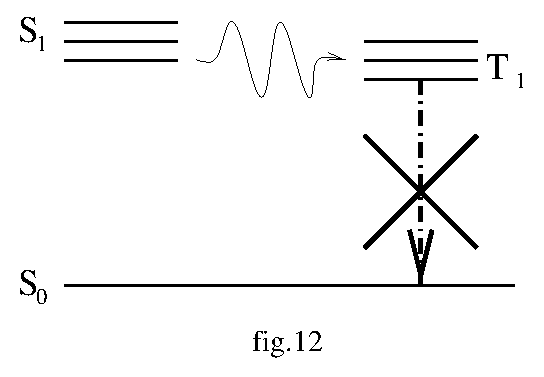
\includegraphics[clip,height=35mm,width=40mm]{1997phy9-16.eps}
\includegraphics[clip,height=35mm,width=40mm]{1997phy9-17.eps}
\end{center}}\parbox[t]{70mm}{金属の3
重項励起状態(fig.13)が$\rm{S_1}$の近くにあると、本来禁制である、1重
項→3重項の遷移が容易に生じる。これをintersystem crossingという。
(fig.12)いったん、これが起こると、基底状態は一重項状態であるから、
$\rm{T_1}$→$\rm{S_0}$は禁制遷移であり、エネルギー差が十分あるので、蛍
光が発生しない(無輻射遷移となるほか、稀に発光過程を行うものもある。)。}

したがって、この『intersystem crossing』に食われる分、蛍光強度は落ちる。
\end{subsubanswers}

%%
\SubAnswer
トリプトファンは蛋白質中の、アミノ酸において、最も強い蛍光を放つ。pH
11 で、最強度となり、励起波長がが287$\mu$\Unit{m}、蛍光波長が
348$\mu$\Unit{m}である。酸性になるにつれ分解が進み、蛍光強度は落ちる。
また、トリプトファンは疎水性である。
\begin{subsubanswers}
\SubSubAnswer

蛋白質は溶媒のpHを減らしていくと、あるpH周辺で急激に立体構造がくずれ、
一次元のひも状となる。この現象をアンフォールディング(unfolding)という
(俗に変性)。蛋白質は3次立体構造をとっているときは、親水部分を外に向け、
疎水性であるトリプトファンは分子内部に詰め込まれる。それがため、構造内
部のトリプトファンは、塩酸グアニジンの影響を受けていない。しかし、アン
フォールディングにより、そういったトリプトファンが一斉に酸性にさらされ
る。そのため、急激にトリプトファン蛍光強度が落ちているのである。

\SubSubAnswer

濃度C${}_0$を超え、トリプトファンが溶媒中にあらわになると、それはトリ
プトファンが溶媒中にある状態となり{\bf{3(ii)}}で述べた影響を受ける。ス
ペクトルは長波長側にシフトする。強度は酸性下のために、低下する。

\end{subsubanswers}
\end{subanswers}
\end{answer}

\end{document}

